% Created by tikzDevice version 0.6.2-92-0ad2792 on 2013-04-20 17:54:59
% !TEX encoding = UTF-8 Unicode
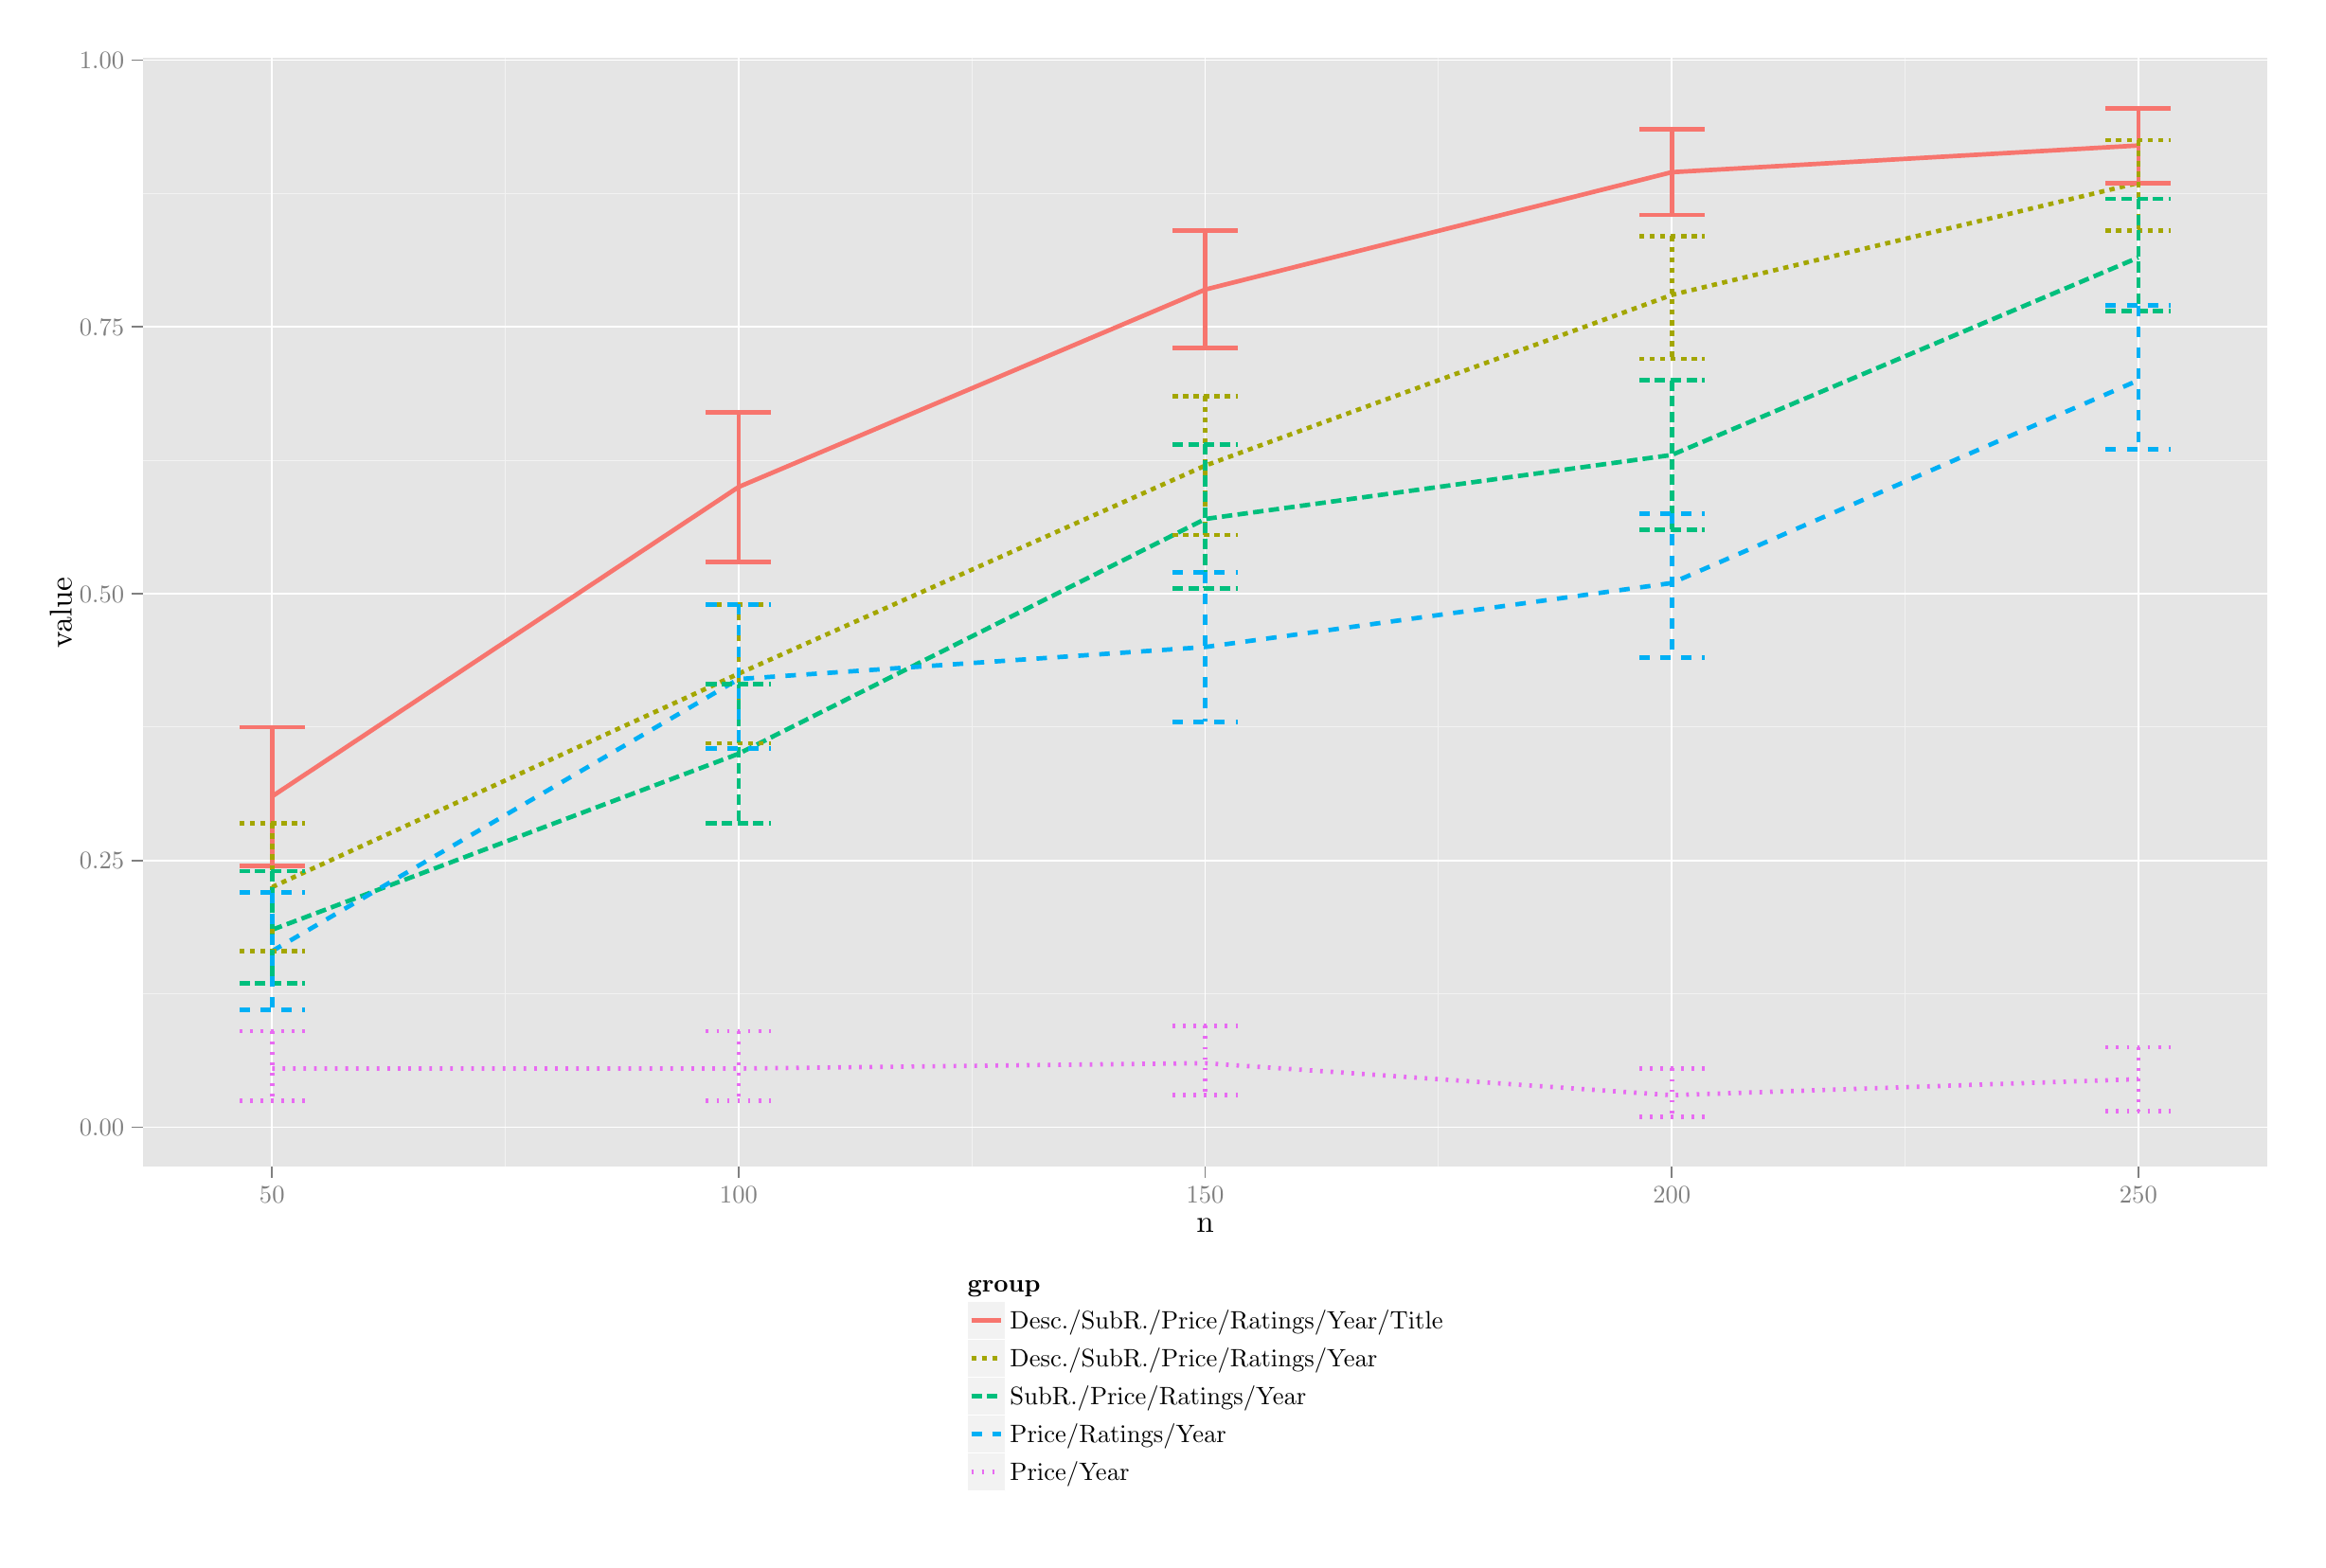
\begin{tikzpicture}[x=1pt,y=1pt]
\definecolor[named]{fillColor}{rgb}{1.00,1.00,1.00}
\path[use as bounding box,fill=fillColor,fill opacity=0.00] (0,0) rectangle (867.24,578.16);
\begin{scope}
\path[clip] (  0.00,  0.00) rectangle (867.24,578.16);
\definecolor[named]{drawColor}{rgb}{1.00,1.00,1.00}
\definecolor[named]{fillColor}{rgb}{1.00,1.00,1.00}

\path[draw=drawColor,line width= 0.6pt,line join=round,line cap=round,fill=fillColor] ( -0.00, -0.00) rectangle (867.24,578.16);
\end{scope}
\begin{scope}
\path[clip] ( 44.49,142.81) rectangle (855.20,566.12);
\definecolor[named]{fillColor}{rgb}{0.90,0.90,0.90}

\path[fill=fillColor] ( 44.49,142.81) rectangle (855.19,566.11);
\definecolor[named]{drawColor}{rgb}{0.95,0.95,0.95}

\path[draw=drawColor,line width= 0.3pt,line join=round] ( 44.49,208.89) --
	(855.20,208.89);

\path[draw=drawColor,line width= 0.3pt,line join=round] ( 44.49,310.69) --
	(855.20,310.69);

\path[draw=drawColor,line width= 0.3pt,line join=round] ( 44.49,412.49) --
	(855.20,412.49);

\path[draw=drawColor,line width= 0.3pt,line join=round] ( 44.49,514.30) --
	(855.20,514.30);

\path[draw=drawColor,line width= 0.3pt,line join=round] (182.81,142.81) --
	(182.81,566.12);

\path[draw=drawColor,line width= 0.3pt,line join=round] (360.83,142.81) --
	(360.83,566.12);

\path[draw=drawColor,line width= 0.3pt,line join=round] (538.85,142.81) --
	(538.85,566.12);

\path[draw=drawColor,line width= 0.3pt,line join=round] (716.87,142.81) --
	(716.87,566.12);
\definecolor[named]{drawColor}{rgb}{1.00,1.00,1.00}

\path[draw=drawColor,line width= 0.6pt,line join=round] ( 44.49,157.98) --
	(855.20,157.98);

\path[draw=drawColor,line width= 0.6pt,line join=round] ( 44.49,259.79) --
	(855.20,259.79);

\path[draw=drawColor,line width= 0.6pt,line join=round] ( 44.49,361.59) --
	(855.20,361.59);

\path[draw=drawColor,line width= 0.6pt,line join=round] ( 44.49,463.39) --
	(855.20,463.39);

\path[draw=drawColor,line width= 0.6pt,line join=round] ( 44.49,565.20) --
	(855.20,565.20);

\path[draw=drawColor,line width= 0.6pt,line join=round] ( 93.80,142.81) --
	( 93.80,566.12);

\path[draw=drawColor,line width= 0.6pt,line join=round] (271.82,142.81) --
	(271.82,566.12);

\path[draw=drawColor,line width= 0.6pt,line join=round] (449.84,142.81) --
	(449.84,566.12);

\path[draw=drawColor,line width= 0.6pt,line join=round] (627.86,142.81) --
	(627.86,566.12);

\path[draw=drawColor,line width= 0.6pt,line join=round] (805.88,142.81) --
	(805.88,566.12);
\definecolor[named]{drawColor}{rgb}{0.97,0.46,0.43}

\path[draw=drawColor,line width= 1.7pt,line join=round] ( 93.80,284.22) --
	(271.82,402.31) --
	(449.84,477.65) --
	(627.86,522.44) --
	(805.88,532.62);
\definecolor[named]{drawColor}{rgb}{0.64,0.65,0.00}

\path[draw=drawColor,line width= 1.7pt,dash pattern=on 2pt off 2pt ,line join=round] ( 93.80,249.61) --
	(271.82,331.05) --
	(449.84,410.46) --
	(627.86,475.61) --
	(805.88,518.37);
\definecolor[named]{drawColor}{rgb}{0.00,0.75,0.49}

\path[draw=drawColor,line width= 1.7pt,dash pattern=on 4pt off 2pt ,line join=round] ( 93.80,233.32) --
	(271.82,300.51) --
	(449.84,390.10) --
	(627.86,414.53) --
	(805.88,489.86);
\definecolor[named]{drawColor}{rgb}{0.00,0.69,0.96}

\path[draw=drawColor,line width= 1.7pt,dash pattern=on 4pt off 4pt ,line join=round] ( 93.80,225.17) --
	(271.82,329.01) --
	(449.84,341.23) --
	(627.86,365.66) --
	(805.88,443.03);
\definecolor[named]{drawColor}{rgb}{0.91,0.42,0.95}

\path[draw=drawColor,line width= 1.7pt,dash pattern=on 1pt off 3pt ,line join=round] ( 93.80,180.38) --
	(271.82,180.38) --
	(449.84,182.42) --
	(627.86,170.20) --
	(805.88,176.31);
\definecolor[named]{drawColor}{rgb}{0.97,0.46,0.43}

\path[draw=drawColor,line width= 1.7pt,line join=round] ( 81.34,310.69) --
	(106.26,310.69);

\path[draw=drawColor,line width= 1.7pt,line join=round] ( 93.80,310.69) --
	( 93.80,257.75);

\path[draw=drawColor,line width= 1.7pt,line join=round] ( 81.34,257.75) --
	(106.26,257.75);

\path[draw=drawColor,line width= 1.7pt,line join=round] (259.36,430.82) --
	(284.28,430.82);

\path[draw=drawColor,line width= 1.7pt,line join=round] (271.82,430.82) --
	(271.82,373.81);

\path[draw=drawColor,line width= 1.7pt,line join=round] (259.36,373.81) --
	(284.28,373.81);

\path[draw=drawColor,line width= 1.7pt,line join=round] (437.38,500.04) --
	(462.30,500.04);

\path[draw=drawColor,line width= 1.7pt,line join=round] (449.84,500.04) --
	(449.84,455.25);

\path[draw=drawColor,line width= 1.7pt,line join=round] (437.38,455.25) --
	(462.30,455.25);

\path[draw=drawColor,line width= 1.7pt,line join=round] (615.40,538.73) --
	(640.32,538.73);

\path[draw=drawColor,line width= 1.7pt,line join=round] (627.86,538.73) --
	(627.86,506.10);

\path[draw=drawColor,line width= 1.7pt,line join=round] (615.40,506.10) --
	(640.32,506.10);

\path[draw=drawColor,line width= 1.7pt,line join=round] (793.42,546.87) --
	(818.34,546.87);

\path[draw=drawColor,line width= 1.7pt,line join=round] (805.88,546.87) --
	(805.88,518.32);

\path[draw=drawColor,line width= 1.7pt,line join=round] (793.42,518.32) --
	(818.34,518.32);
\definecolor[named]{drawColor}{rgb}{0.64,0.65,0.00}

\path[draw=drawColor,line width= 1.7pt,dash pattern=on 2pt off 2pt ,line join=round] ( 81.34,274.04) --
	(106.26,274.04);

\path[draw=drawColor,line width= 1.7pt,dash pattern=on 2pt off 2pt ,line join=round] ( 93.80,274.04) --
	( 93.80,225.17);

\path[draw=drawColor,line width= 1.7pt,dash pattern=on 2pt off 2pt ,line join=round] ( 81.34,225.17) --
	(106.26,225.17);

\path[draw=drawColor,line width= 1.7pt,dash pattern=on 2pt off 2pt ,line join=round] (259.36,357.52) --
	(284.28,357.52);

\path[draw=drawColor,line width= 1.7pt,dash pattern=on 2pt off 2pt ,line join=round] (271.82,357.52) --
	(271.82,304.53);

\path[draw=drawColor,line width= 1.7pt,dash pattern=on 2pt off 2pt ,line join=round] (259.36,304.53) --
	(284.28,304.53);

\path[draw=drawColor,line width= 1.7pt,dash pattern=on 2pt off 2pt ,line join=round] (437.38,436.93) --
	(462.30,436.93);

\path[draw=drawColor,line width= 1.7pt,dash pattern=on 2pt off 2pt ,line join=round] (449.84,436.93) --
	(449.84,383.99);

\path[draw=drawColor,line width= 1.7pt,dash pattern=on 2pt off 2pt ,line join=round] (437.38,383.99) --
	(462.30,383.99);

\path[draw=drawColor,line width= 1.7pt,dash pattern=on 2pt off 2pt ,line join=round] (615.40,498.01) --
	(640.32,498.01);

\path[draw=drawColor,line width= 1.7pt,dash pattern=on 2pt off 2pt ,line join=round] (627.86,498.01) --
	(627.86,451.18);

\path[draw=drawColor,line width= 1.7pt,dash pattern=on 2pt off 2pt ,line join=round] (615.40,451.18) --
	(640.32,451.18);

\path[draw=drawColor,line width= 1.7pt,dash pattern=on 2pt off 2pt ,line join=round] (793.42,534.66) --
	(818.34,534.66);

\path[draw=drawColor,line width= 1.7pt,dash pattern=on 2pt off 2pt ,line join=round] (805.88,534.66) --
	(805.88,500.04);

\path[draw=drawColor,line width= 1.7pt,dash pattern=on 2pt off 2pt ,line join=round] (793.42,500.04) --
	(818.34,500.04);
\definecolor[named]{drawColor}{rgb}{0.00,0.75,0.49}

\path[draw=drawColor,line width= 1.7pt,dash pattern=on 4pt off 2pt ,line join=round] ( 81.34,255.72) --
	(106.26,255.72);

\path[draw=drawColor,line width= 1.7pt,dash pattern=on 4pt off 2pt ,line join=round] ( 93.80,255.72) --
	( 93.80,212.91);

\path[draw=drawColor,line width= 1.7pt,dash pattern=on 4pt off 2pt ,line join=round] ( 81.34,212.91) --
	(106.26,212.91);

\path[draw=drawColor,line width= 1.7pt,dash pattern=on 4pt off 2pt ,line join=round] (259.36,326.98) --
	(284.28,326.98);

\path[draw=drawColor,line width= 1.7pt,dash pattern=on 4pt off 2pt ,line join=round] (271.82,326.98) --
	(271.82,274.04);

\path[draw=drawColor,line width= 1.7pt,dash pattern=on 4pt off 2pt ,line join=round] (259.36,274.04) --
	(284.28,274.04);

\path[draw=drawColor,line width= 1.7pt,dash pattern=on 4pt off 2pt ,line join=round] (437.38,418.60) --
	(462.30,418.60);

\path[draw=drawColor,line width= 1.7pt,dash pattern=on 4pt off 2pt ,line join=round] (449.84,418.60) --
	(449.84,363.58);

\path[draw=drawColor,line width= 1.7pt,dash pattern=on 4pt off 2pt ,line join=round] (437.38,363.58) --
	(462.30,363.58);

\path[draw=drawColor,line width= 1.7pt,dash pattern=on 4pt off 2pt ,line join=round] (615.40,443.03) --
	(640.32,443.03);

\path[draw=drawColor,line width= 1.7pt,dash pattern=on 4pt off 2pt ,line join=round] (627.86,443.03) --
	(627.86,386.02);

\path[draw=drawColor,line width= 1.7pt,dash pattern=on 4pt off 2pt ,line join=round] (615.40,386.02) --
	(640.32,386.02);

\path[draw=drawColor,line width= 1.7pt,dash pattern=on 4pt off 2pt ,line join=round] (793.42,512.26) --
	(818.34,512.26);

\path[draw=drawColor,line width= 1.7pt,dash pattern=on 4pt off 2pt ,line join=round] (805.88,512.26) --
	(805.88,469.50);

\path[draw=drawColor,line width= 1.7pt,dash pattern=on 4pt off 2pt ,line join=round] (793.42,469.50) --
	(818.34,469.50);
\definecolor[named]{drawColor}{rgb}{0.00,0.69,0.96}

\path[draw=drawColor,line width= 1.7pt,dash pattern=on 4pt off 4pt ,line join=round] ( 81.34,247.57) --
	(106.26,247.57);

\path[draw=drawColor,line width= 1.7pt,dash pattern=on 4pt off 4pt ,line join=round] ( 93.80,247.57) --
	( 93.80,202.78);

\path[draw=drawColor,line width= 1.7pt,dash pattern=on 4pt off 4pt ,line join=round] ( 81.34,202.78) --
	(106.26,202.78);

\path[draw=drawColor,line width= 1.7pt,dash pattern=on 4pt off 4pt ,line join=round] (259.36,357.52) --
	(284.28,357.52);

\path[draw=drawColor,line width= 1.7pt,dash pattern=on 4pt off 4pt ,line join=round] (271.82,357.52) --
	(271.82,302.54);

\path[draw=drawColor,line width= 1.7pt,dash pattern=on 4pt off 4pt ,line join=round] (259.36,302.54) --
	(284.28,302.54);

\path[draw=drawColor,line width= 1.7pt,dash pattern=on 4pt off 4pt ,line join=round] (437.38,369.74) --
	(462.30,369.74);

\path[draw=drawColor,line width= 1.7pt,dash pattern=on 4pt off 4pt ,line join=round] (449.84,369.74) --
	(449.84,312.73);

\path[draw=drawColor,line width= 1.7pt,dash pattern=on 4pt off 4pt ,line join=round] (437.38,312.73) --
	(462.30,312.73);

\path[draw=drawColor,line width= 1.7pt,dash pattern=on 4pt off 4pt ,line join=round] (615.40,392.18) --
	(640.32,392.18);

\path[draw=drawColor,line width= 1.7pt,dash pattern=on 4pt off 4pt ,line join=round] (627.86,392.18) --
	(627.86,337.16);

\path[draw=drawColor,line width= 1.7pt,dash pattern=on 4pt off 4pt ,line join=round] (615.40,337.16) --
	(640.32,337.16);

\path[draw=drawColor,line width= 1.7pt,dash pattern=on 4pt off 4pt ,line join=round] (793.42,471.54) --
	(818.34,471.54);

\path[draw=drawColor,line width= 1.7pt,dash pattern=on 4pt off 4pt ,line join=round] (805.88,471.54) --
	(805.88,416.57);

\path[draw=drawColor,line width= 1.7pt,dash pattern=on 4pt off 4pt ,line join=round] (793.42,416.57) --
	(818.34,416.57);
\definecolor[named]{drawColor}{rgb}{0.91,0.42,0.95}

\path[draw=drawColor,line width= 1.7pt,dash pattern=on 1pt off 3pt ,line join=round] ( 81.34,194.63) --
	(106.26,194.63);

\path[draw=drawColor,line width= 1.7pt,dash pattern=on 1pt off 3pt ,line join=round] ( 93.80,194.63) --
	( 93.80,168.16);

\path[draw=drawColor,line width= 1.7pt,dash pattern=on 1pt off 3pt ,line join=round] ( 81.34,168.16) --
	(106.26,168.16);

\path[draw=drawColor,line width= 1.7pt,dash pattern=on 1pt off 3pt ,line join=round] (259.36,194.63) --
	(284.28,194.63);

\path[draw=drawColor,line width= 1.7pt,dash pattern=on 1pt off 3pt ,line join=round] (271.82,194.63) --
	(271.82,168.16);

\path[draw=drawColor,line width= 1.7pt,dash pattern=on 1pt off 3pt ,line join=round] (259.36,168.16) --
	(284.28,168.16);

\path[draw=drawColor,line width= 1.7pt,dash pattern=on 1pt off 3pt ,line join=round] (437.38,196.67) --
	(462.30,196.67);

\path[draw=drawColor,line width= 1.7pt,dash pattern=on 1pt off 3pt ,line join=round] (449.84,196.67) --
	(449.84,170.20);

\path[draw=drawColor,line width= 1.7pt,dash pattern=on 1pt off 3pt ,line join=round] (437.38,170.20) --
	(462.30,170.20);

\path[draw=drawColor,line width= 1.7pt,dash pattern=on 1pt off 3pt ,line join=round] (615.40,180.38) --
	(640.32,180.38);

\path[draw=drawColor,line width= 1.7pt,dash pattern=on 1pt off 3pt ,line join=round] (627.86,180.38) --
	(627.86,162.06);

\path[draw=drawColor,line width= 1.7pt,dash pattern=on 1pt off 3pt ,line join=round] (615.40,162.06) --
	(640.32,162.06);

\path[draw=drawColor,line width= 1.7pt,dash pattern=on 1pt off 3pt ,line join=round] (793.42,188.52) --
	(818.34,188.52);

\path[draw=drawColor,line width= 1.7pt,dash pattern=on 1pt off 3pt ,line join=round] (805.88,188.52) --
	(805.88,164.09);

\path[draw=drawColor,line width= 1.7pt,dash pattern=on 1pt off 3pt ,line join=round] (793.42,164.09) --
	(818.34,164.09);
\end{scope}
\begin{scope}
\path[clip] (  0.00,  0.00) rectangle (867.24,578.16);
\definecolor[named]{drawColor}{rgb}{0.50,0.50,0.50}

\node[text=drawColor,anchor=base east,inner sep=0pt, outer sep=0pt, scale=  0.96] at ( 37.37,154.68) {0.00};

\node[text=drawColor,anchor=base east,inner sep=0pt, outer sep=0pt, scale=  0.96] at ( 37.37,256.48) {0.25};

\node[text=drawColor,anchor=base east,inner sep=0pt, outer sep=0pt, scale=  0.96] at ( 37.37,358.29) {0.50};

\node[text=drawColor,anchor=base east,inner sep=0pt, outer sep=0pt, scale=  0.96] at ( 37.37,460.09) {0.75};

\node[text=drawColor,anchor=base east,inner sep=0pt, outer sep=0pt, scale=  0.96] at ( 37.37,561.89) {1.00};
\end{scope}
\begin{scope}
\path[clip] (  0.00,  0.00) rectangle (867.24,578.16);
\definecolor[named]{drawColor}{rgb}{0.50,0.50,0.50}

\path[draw=drawColor,line width= 0.6pt,line join=round] ( 40.22,157.98) --
	( 44.49,157.98);

\path[draw=drawColor,line width= 0.6pt,line join=round] ( 40.22,259.79) --
	( 44.49,259.79);

\path[draw=drawColor,line width= 0.6pt,line join=round] ( 40.22,361.59) --
	( 44.49,361.59);

\path[draw=drawColor,line width= 0.6pt,line join=round] ( 40.22,463.39) --
	( 44.49,463.39);

\path[draw=drawColor,line width= 0.6pt,line join=round] ( 40.22,565.20) --
	( 44.49,565.20);
\end{scope}
\begin{scope}
\path[clip] (  0.00,  0.00) rectangle (867.24,578.16);
\definecolor[named]{drawColor}{rgb}{0.50,0.50,0.50}

\path[draw=drawColor,line width= 0.6pt,line join=round] ( 93.80,138.55) --
	( 93.80,142.81);

\path[draw=drawColor,line width= 0.6pt,line join=round] (271.82,138.55) --
	(271.82,142.81);

\path[draw=drawColor,line width= 0.6pt,line join=round] (449.84,138.55) --
	(449.84,142.81);

\path[draw=drawColor,line width= 0.6pt,line join=round] (627.86,138.55) --
	(627.86,142.81);

\path[draw=drawColor,line width= 0.6pt,line join=round] (805.88,138.55) --
	(805.88,142.81);
\end{scope}
\begin{scope}
\path[clip] (  0.00,  0.00) rectangle (867.24,578.16);
\definecolor[named]{drawColor}{rgb}{0.50,0.50,0.50}

\node[text=drawColor,anchor=base,inner sep=0pt, outer sep=0pt, scale=  0.96] at ( 93.80,129.09) {50};

\node[text=drawColor,anchor=base,inner sep=0pt, outer sep=0pt, scale=  0.96] at (271.82,129.09) {100};

\node[text=drawColor,anchor=base,inner sep=0pt, outer sep=0pt, scale=  0.96] at (449.84,129.09) {150};

\node[text=drawColor,anchor=base,inner sep=0pt, outer sep=0pt, scale=  0.96] at (627.86,129.09) {200};

\node[text=drawColor,anchor=base,inner sep=0pt, outer sep=0pt, scale=  0.96] at (805.88,129.09) {250};
\end{scope}
\begin{scope}
\path[clip] (  0.00,  0.00) rectangle (867.24,578.16);
\definecolor[named]{drawColor}{rgb}{0.00,0.00,0.00}

\node[text=drawColor,anchor=base,inner sep=0pt, outer sep=0pt, scale=  1.20] at (449.84,117.81) {n};
\end{scope}
\begin{scope}
\path[clip] (  0.00,  0.00) rectangle (867.24,578.16);
\definecolor[named]{drawColor}{rgb}{0.00,0.00,0.00}

\node[text=drawColor,rotate= 90.00,anchor=base,inner sep=0pt, outer sep=0pt, scale=  1.20] at ( 17.30,354.46) {value};
\end{scope}
\begin{scope}
\path[clip] (  0.00,  0.00) rectangle (867.24,578.16);
\definecolor[named]{fillColor}{rgb}{1.00,1.00,1.00}

\path[fill=fillColor] (354.85, 14.89) rectangle (544.83,105.93);
\end{scope}
\begin{scope}
\path[clip] (  0.00,  0.00) rectangle (867.24,578.16);
\definecolor[named]{drawColor}{rgb}{0.00,0.00,0.00}

\node[text=drawColor,anchor=base west,inner sep=0pt, outer sep=0pt, scale=  0.96] at (359.12, 95.04) {\bfseries group};
\end{scope}
\begin{scope}
\path[clip] (  0.00,  0.00) rectangle (867.24,578.16);
\definecolor[named]{drawColor}{rgb}{1.00,1.00,1.00}
\definecolor[named]{fillColor}{rgb}{0.95,0.95,0.95}

\path[draw=drawColor,line width= 0.6pt,line join=round,line cap=round,fill=fillColor] (359.12, 76.97) rectangle (373.57, 91.43);
\end{scope}
\begin{scope}
\path[clip] (  0.00,  0.00) rectangle (867.24,578.16);
\definecolor[named]{drawColor}{rgb}{0.97,0.46,0.43}

\path[draw=drawColor,line width= 1.7pt,line join=round] (360.56, 84.20) -- (372.12, 84.20);
\end{scope}
\begin{scope}
\path[clip] (  0.00,  0.00) rectangle (867.24,578.16);
\definecolor[named]{drawColor}{rgb}{0.97,0.46,0.43}

\path[draw=drawColor,line width= 1.7pt,line join=round] (360.56, 84.20) -- (372.12, 84.20);
\end{scope}
\begin{scope}
\path[clip] (  0.00,  0.00) rectangle (867.24,578.16);
\definecolor[named]{drawColor}{rgb}{1.00,1.00,1.00}
\definecolor[named]{fillColor}{rgb}{0.95,0.95,0.95}

\path[draw=drawColor,line width= 0.6pt,line join=round,line cap=round,fill=fillColor] (359.12, 62.52) rectangle (373.57, 76.97);
\end{scope}
\begin{scope}
\path[clip] (  0.00,  0.00) rectangle (867.24,578.16);
\definecolor[named]{drawColor}{rgb}{0.64,0.65,0.00}

\path[draw=drawColor,line width= 1.7pt,dash pattern=on 2pt off 2pt ,line join=round] (360.56, 69.75) -- (372.12, 69.75);
\end{scope}
\begin{scope}
\path[clip] (  0.00,  0.00) rectangle (867.24,578.16);
\definecolor[named]{drawColor}{rgb}{0.64,0.65,0.00}

\path[draw=drawColor,line width= 1.7pt,dash pattern=on 2pt off 2pt ,line join=round] (360.56, 69.75) -- (372.12, 69.75);
\end{scope}
\begin{scope}
\path[clip] (  0.00,  0.00) rectangle (867.24,578.16);
\definecolor[named]{drawColor}{rgb}{1.00,1.00,1.00}
\definecolor[named]{fillColor}{rgb}{0.95,0.95,0.95}

\path[draw=drawColor,line width= 0.6pt,line join=round,line cap=round,fill=fillColor] (359.12, 48.07) rectangle (373.57, 62.52);
\end{scope}
\begin{scope}
\path[clip] (  0.00,  0.00) rectangle (867.24,578.16);
\definecolor[named]{drawColor}{rgb}{0.00,0.75,0.49}

\path[draw=drawColor,line width= 1.7pt,dash pattern=on 4pt off 2pt ,line join=round] (360.56, 55.29) -- (372.12, 55.29);
\end{scope}
\begin{scope}
\path[clip] (  0.00,  0.00) rectangle (867.24,578.16);
\definecolor[named]{drawColor}{rgb}{0.00,0.75,0.49}

\path[draw=drawColor,line width= 1.7pt,dash pattern=on 4pt off 2pt ,line join=round] (360.56, 55.29) -- (372.12, 55.29);
\end{scope}
\begin{scope}
\path[clip] (  0.00,  0.00) rectangle (867.24,578.16);
\definecolor[named]{drawColor}{rgb}{1.00,1.00,1.00}
\definecolor[named]{fillColor}{rgb}{0.95,0.95,0.95}

\path[draw=drawColor,line width= 0.6pt,line join=round,line cap=round,fill=fillColor] (359.12, 33.61) rectangle (373.57, 48.07);
\end{scope}
\begin{scope}
\path[clip] (  0.00,  0.00) rectangle (867.24,578.16);
\definecolor[named]{drawColor}{rgb}{0.00,0.69,0.96}

\path[draw=drawColor,line width= 1.7pt,dash pattern=on 4pt off 4pt ,line join=round] (360.56, 40.84) -- (372.12, 40.84);
\end{scope}
\begin{scope}
\path[clip] (  0.00,  0.00) rectangle (867.24,578.16);
\definecolor[named]{drawColor}{rgb}{0.00,0.69,0.96}

\path[draw=drawColor,line width= 1.7pt,dash pattern=on 4pt off 4pt ,line join=round] (360.56, 40.84) -- (372.12, 40.84);
\end{scope}
\begin{scope}
\path[clip] (  0.00,  0.00) rectangle (867.24,578.16);
\definecolor[named]{drawColor}{rgb}{1.00,1.00,1.00}
\definecolor[named]{fillColor}{rgb}{0.95,0.95,0.95}

\path[draw=drawColor,line width= 0.6pt,line join=round,line cap=round,fill=fillColor] (359.12, 19.16) rectangle (373.57, 33.61);
\end{scope}
\begin{scope}
\path[clip] (  0.00,  0.00) rectangle (867.24,578.16);
\definecolor[named]{drawColor}{rgb}{0.91,0.42,0.95}

\path[draw=drawColor,line width= 1.7pt,dash pattern=on 1pt off 3pt ,line join=round] (360.56, 26.39) -- (372.12, 26.39);
\end{scope}
\begin{scope}
\path[clip] (  0.00,  0.00) rectangle (867.24,578.16);
\definecolor[named]{drawColor}{rgb}{0.91,0.42,0.95}

\path[draw=drawColor,line width= 1.7pt,dash pattern=on 1pt off 3pt ,line join=round] (360.56, 26.39) -- (372.12, 26.39);
\end{scope}
\begin{scope}
\path[clip] (  0.00,  0.00) rectangle (867.24,578.16);
\definecolor[named]{drawColor}{rgb}{0.00,0.00,0.00}

\node[text=drawColor,anchor=base west,inner sep=0pt, outer sep=0pt, scale=  0.96] at (375.38, 80.90) {Desc./SubR./Price/Ratings/Year/Title};
\end{scope}
\begin{scope}
\path[clip] (  0.00,  0.00) rectangle (867.24,578.16);
\definecolor[named]{drawColor}{rgb}{0.00,0.00,0.00}

\node[text=drawColor,anchor=base west,inner sep=0pt, outer sep=0pt, scale=  0.96] at (375.38, 66.44) {Desc./SubR./Price/Ratings/Year};
\end{scope}
\begin{scope}
\path[clip] (  0.00,  0.00) rectangle (867.24,578.16);
\definecolor[named]{drawColor}{rgb}{0.00,0.00,0.00}

\node[text=drawColor,anchor=base west,inner sep=0pt, outer sep=0pt, scale=  0.96] at (375.38, 51.99) {SubR./Price/Ratings/Year};
\end{scope}
\begin{scope}
\path[clip] (  0.00,  0.00) rectangle (867.24,578.16);
\definecolor[named]{drawColor}{rgb}{0.00,0.00,0.00}

\node[text=drawColor,anchor=base west,inner sep=0pt, outer sep=0pt, scale=  0.96] at (375.38, 37.53) {Price/Ratings/Year};
\end{scope}
\begin{scope}
\path[clip] (  0.00,  0.00) rectangle (867.24,578.16);
\definecolor[named]{drawColor}{rgb}{0.00,0.00,0.00}

\node[text=drawColor,anchor=base west,inner sep=0pt, outer sep=0pt, scale=  0.96] at (375.38, 23.08) {Price/Year};
\end{scope}
\end{tikzpicture}
